\section{What training buys: controlled campaigns}
\label{sec:campaigns}
\label{sec:res-primary}

Released dictionaries tell us what trained codes look like; they cannot tell us what any particular
choice during training does to them, because nothing about them was under our control. This section
supplies the intervention. We train 400 small networks in which the loss, the width, the feature load
and the training sparsity are set by us, measure the same statistics on the resulting codes, and
retain every trained model so that later analyses need no retraining --- three of the results below
were computed months after the runs, from the saved weights alone.

\subsection{The network against an affine probe of its own representation}

The campaigns in Appendix~\ref{app:earlier} compare the network's thresholded output against
\emph{fixed} readouts of its code. That understates the baseline, and the audit that prompted this
campaign said so. Stage A replaces it: 180 models at $d\in\{50,100,200\}$ with $F=2d$, 20 seeds per cell, three code families
($L^4$, $L^2$, and an untrained random code), and an affine probe fitted over three families, two
representations, three threshold policies and a six-point regularisation grid, all selected on
validation with the test split opened once. \code{tests/test\_probes.py} poisons the test set and
asserts that no selected hyperparameter moves, so leakage is excluded structurally rather than by
inspection.

\paragraph{Splits, and where they cannot be disjoint.} Train, validation and test draw
\emph{disjoint supports}, which is a stronger guarantee than disjoint states and is what makes a
fitted probe's test score meaningful. It cannot hold unconditionally: at $s=1$ there are only $F$
supports in total --- 100, 200 and 400 at the three widths --- against the thousands of states each
split requests. The sampler therefore serves the test split first, caps the smallest sparsities at
what the space contains, and distributes the remainder proportionally; it records which sparsities
were exhausted and how many draws were rejected, and it raises rather than silently returning an
empty split. At $F=100$ the $s=1$ test set holds 50 states, not 4096, and the sparsities $s\in\{1,2\}$
are flagged exhausted. Every per-sparsity rate at those sparsities is therefore computed on fewer
states than the nominal budget, and its Wilson interval is correspondingly wider.

\paragraph{The comparison has to be matched, and matching it changes the answer.}
A first pass compared the network at a fixed $\theta=1/2$ against the best of all eighteen probe
configurations. That stacks three advantages on the probe: two thirds of the configurations tune
their threshold on validation while the network does not; two thirds read the \emph{pre}-ReLU state
$\Phi b$ while the network's output layer reads $\mathrm{ReLU}(\Phi b)$; and $\theta=1/2$ is not on a
common scale across a ridge prediction, a logistic probability and a hinge margin. Removing all
three --- probe restricted to the post-ReLU state, one validation-selected global threshold for each
side, differences paired within seed --- gives Table~\ref{tab:primary}.

\begin{table}[t]
\centering
\caption{The matched comparison: network minus best post-ReLU affine probe in $s_{95}$, paired
within seed, with a bootstrap interval over the models of each cell (20 at $d\le200$, \ScSeeds{} at
$d=400$). Both decoders read the same state and each gets one validation-selected global threshold.
The sign is a property of the code and not of the protocol: positive for $L^4$ and growing with
width, exactly zero for $L^2$ --- where both decoders are at $s_{95}=0$ and the zero is a joint
failure rather than an agreement --- and strongly negative for an untrained code, under the identical
procedure. Section~\ref{sec:probes} states what the comparison can and cannot mean. Generated from
\texttt{results/e7/derived/} and \texttt{results/e7\_stageC/derived/}.}
\label{tab:primary}
\small
% Generated by scripts/make_tables.py from results/. Do not edit by hand.
\begin{tabular}{llcccc}
\toprule
code & $d$ & mean difference & 95\% interval & net / tie / probe & AUC difference \\
\midrule
$L^4$ & 50 & +0.00 & [+0.00, +0.00] & 0 / 20 / 0 & +0.0053 \\
$L^4$ & 100 & +0.35 & [+0.05, +0.60] & 9 / 9 / 2 & +0.0210 \\
$L^4$ & 200 & +0.35 & [+0.10, +0.60] & 6 / 14 / 0 & +0.0379 \\
$L^4$ & 400 & +2.00 & [+1.50, +2.50] & 10 / 0 / 0 & +0.0699 \\
\addlinespace[3pt]
$L^2$ & 50 & +0.00 & [+0.00, +0.00] & 0 / 20 / 0 & +0.0007 \\
$L^2$ & 100 & +0.00 & [+0.00, +0.00] & 0 / 20 / 0 & +0.0004 \\
$L^2$ & 200 & +0.00 & [+0.00, +0.00] & 0 / 20 / 0 & +0.0007 \\
$L^2$ & 400 & +0.00 & [+0.00, +0.00] & 0 / 10 / 0 & +0.0008 \\
\addlinespace[3pt]
untrained & 50 & -1.00 & [-1.00, -1.00] & 0 / 0 / 20 & -0.2122 \\
untrained & 100 & -2.00 & [-2.00, -2.00] & 0 / 0 / 20 & -0.2098 \\
untrained & 200 & -2.30 & [-2.50, -2.10] & 0 / 0 / 20 & -0.1805 \\
untrained & 400 & -2.60 & [-3.10, -2.10] & 0 / 0 / 10 & -0.1782 \\
\bottomrule
\end{tabular}

\end{table}

Across the \PrimModels{} trained models the two tie in \PrimTies, with \PrimNetWins{} models where
the network leads and \PrimProbeWins{} where the probe does. That single count needs breaking down
before it is read, because \PrimLtwoJointFailures{} of the ties are $L^2$ cells in which both
decoders sit at $s_{95}=0$: those are joint failures, not agreements, and counting them as ties
inflates the apparent evidence for equivalence. Among the \PrimLfourModels{} $L^4$ models the split
is \PrimLfourTies{} ties, \PrimNetWins{} to the network and \PrimProbeWins{} to the probe, and the
difference grows with width.

The registered outcome was that a properly trained, validation-selected affine decoder would
\emph{match} the network, and at the smallest width it does. It stops doing so as width grows. We
report that, and Section~\ref{sec:probes} states what the comparison can and cannot mean, because
the probe class contains the network's own decoder and the gap therefore measures the fitting
procedure rather than the expressiveness of affine maps.

\paragraph{The sign is set by the code, not by the protocol.} The obvious objection to the paragraph
above is that a protocol giving both sides a validation-selected threshold must end up favouring the
network, which has one output layer to calibrate against the probe's eighteen configurations. The
untrained arm answers it. Run through the identical procedure, an untrained code's own thresholded
readout \emph{loses} to the fitted affine probe by \PrimRandFiftyDiff{}, \PrimRandHundredDiff{},
\PrimRandTwoHundredDiff{} and \PrimRandFourHundredDiff{} sparsity levels at the four widths, on every
one of the \PrimRandTwoHundredProbeWins{} models per cell at $d\le200$ and all
\PrimRandFourHundredProbeWins{} at $d=400$, with AUC differences of \PrimRandFiftyAucDiff{} to
\PrimRandFourHundredAucDiff{} --- two orders of magnitude larger than any $L^4$ cell and in the
opposite direction. A procedure that systematically favoured the network could not produce that.

So across the three code families the same protocol gives three different answers, and which one it
gives is decided by how the code was made: the network leads under $L^4$ and increasingly with width,
neither decoder recovers anything under $L^2$, and the probe leads by a wide margin on a code that
was never trained. Read as a decoder comparison this table says little; read as a property of the
code, the ordering is the result.

\paragraph{The second estimand agrees, and the earlier disagreement was an artefact.} The analysis
plan named two co-primary estimands: $s_{95}$ and the recovery AUC, the area under the exact-recovery
curve over the evaluated sparsities. $s_{95}$ is a floored crossing point and therefore blunt, so a
difference of less than one level is invisible to it; the AUC sees the whole curve. On the same
matched post-ReLU comparison the AUC is positive at every width and grows with it:
\AucFiftyDiff{} (95\% interval [\AucFiftyCiLow, \AucFiftyCiHigh]) on \AucFiftyNetWins{} of
\EsevenSeeds{} seeds at $d=50$; \AucHundredDiff{} ([\AucHundredCiLow, \AucHundredCiHigh]) on
\AucHundredNetWins{} of \EsevenSeeds{} at $d=100$; \AucTwoHundredDiff{}
([\AucTwoHundredCiLow, \AucTwoHundredCiHigh]) on \AucTwoHundredNetWins{} of \EsevenSeeds{} at
$d=200$; and \AucFourHundredDiff{}
([\AucFourHundredCiLow, \AucFourHundredCiHigh]) on \AucFourHundredNetWins{} of \ScSeeds{} at
$d=400$. Every cell is unanimous across seeds and no interval covers zero.

An earlier version of this section reported the opposite: an AUC that changed sign with width, which
we described as the two estimands disagreeing and treated as the finding. That reading was produced
by a defect in how the shared threshold was selected (Appendix~\ref{app:withdrawn}), which cost the
network up to five sparsity levels at the widest setting. With the defect fixed the two estimands
concur, and their concurrence is the more informative outcome: a difference visible to a blunt
statistic and to a fine one, in the same direction, is harder to attribute to the choice of summary.
Figure~\ref{fig:e7primary}(a,b)
shows both estimands at all four widths so that a reader can see the agreement rather than take our
word for it.

\paragraph{The nonlinearity costs almost nothing on a trained code, and a great deal on an
untrained one.} Restoring the pre-ReLU probe --- which reads the preactivation $\Phi b$, a state the
network's output layer never sees --- is how we had previously located the effect, and on the $L^4$
codes it now finds very little. The pre-ReLU probe's advantage is \PrimLfourFiftyPreDiff{} of a
sparsity level at $d=50$ with \PrimLfourFiftyPreTies{} of \EsevenSeeds{} seeds tied,
\PrimLfourHundredPreDiff{} at $d=100$, \PrimLfourTwoHundredPreDiff{} at $d=200$, and at $d=400$ it
reverses sign: the network leads even the pre-ReLU probe by \PrimLfourFourHundredPreDiff{} on
\PrimLfourFourHundredPreNetWins{} of \ScSeeds{} models. An earlier version of this paper read a
full-level gap here as a measurement of what the ReLU discards; that reading was an artefact of the
threshold defect and is withdrawn (Appendix~\ref{app:withdrawn}, item 2).

On the untrained arm the same comparison is an order of magnitude larger and unanimous:
\PrimRandFiftyPreDiff{}, \PrimRandHundredPreDiff{}, \PrimRandTwoHundredPreDiff{} and
\PrimRandFourHundredPreDiff{} levels to the pre-ReLU probe, growing steeply with width. So the
pipeline of ReLU plus a single global threshold throws away a large and growing amount of affinely
accessible information on a code that was never trained, and next to none on one trained under
$L^4$. That is the surviving form of the claim, and it is a statement about the interaction between
the code and the readout rather than about the nonlinearity alone.

\begin{figure}[t]
\centering
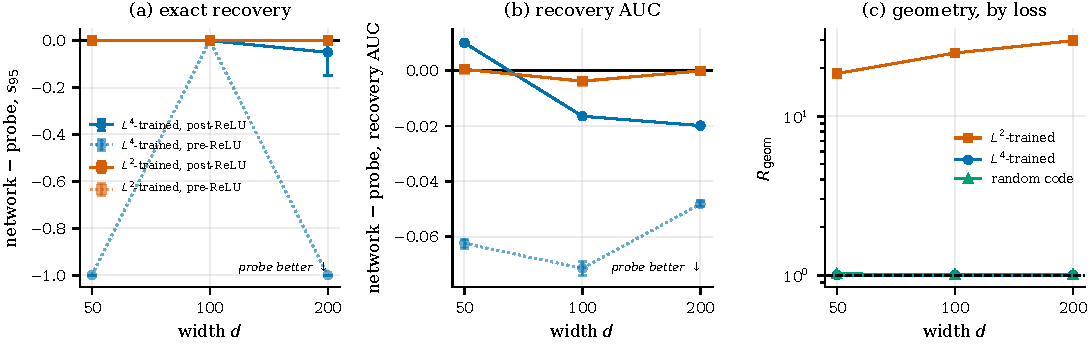
\includegraphics[width=\linewidth]{figures/fig5_matched_comparison.pdf}
\caption{\textbf{The matched comparison, both estimands, and the geometry the loss produces.}
Paired within seed; bars are bootstrap intervals over the models of a cell. Negative means the affine
probe decodes better. \textbf{(a)} Under $s_{95}$ the matched post-ReLU comparison separates the three
code families in three directions: the network leads under $L^4$ by an amount that grows with width,
$L^2$ is a flat zero because neither decoder recovers anything, and on an untrained code the probe
leads by one to two and a half levels. The protocol is identical in all three.
\textbf{(b)} The same models under the recovery AUC, which resolves differences smaller than one
sparsity level and agrees with $s_{95}$ at every width --- an earlier version reported a sign reversal
here, which was an artefact of the threshold defect (Appendix~\ref{app:withdrawn}).
\textbf{(c)} $R_{\mathrm{geom}}$ by loss. $L^2$ leaves the interface one to two orders of magnitude
above the rank--trace floor; $L^4$ and an \emph{untrained} random code both sit on it, which is why
proximity to the floor is not by itself evidence of learned structure.}
\label{fig:e7primary}
\end{figure}

\paragraph{The loss decides the interface.} The three code families separate cleanly and by a wide
margin, at every width:

\begin{center}\small
\begin{tabular}{lccc}
\toprule
& $d=50$ & $d=100$ & $d=200$ \\
\midrule
$R_{\mathrm{geom}}$, $L^4$ & \SALfourFiftyRgeom & \SALfourHundredRgeom & \SALfourTwoHundredRgeom \\
$R_{\mathrm{geom}}$, $L^2$ & \SALtwoFiftyRgeom & \SALtwoHundredRgeom & \SALtwoTwoHundredRgeom \\
$R_{\mathrm{geom}}$, random & \SARandFiftyRgeom & \SARandHundredRgeom & \SARandTwoHundredRgeom \\
\midrule
$\kappa_{\min}$, $L^4$ & \FullLfourFiftyKappaMin & \FullLfourHundredKappaMin & \FullLfourTwoHundredKappaMin \\
$\kappa_{\min}$, $L^2$ & \FullLtwoFiftyKappaMin & \FullLtwoHundredKappaMin & \FullLtwoTwoHundredKappaMin \\
$\kappa_{\min}$, random & \FullRandFiftyKappaMin & \FullRandHundredKappaMin & \FullRandTwoHundredKappaMin \\
\bottomrule
\end{tabular}
\end{center}

$L^2$ drives $R_{\mathrm{geom}}$ into the tens and rising with width, and its frontier collapses to
$1$ --- by Theorem~\ref{thm:frontier} some feature is not separable even at $s=1$, which for
singleton states means two features share a representation. The mechanism is a spread of column
norms: a feature whose direction is a fraction of a typical length lies inside the convex hull of
the others, and no duplicate is needed. $L^4$ does not do this, and its
$R_{\mathrm{readout}}$ of \SALfourFiftyRreadout{} says its own output layer is near-optimal for the
code it built.

\paragraph{But near-floor geometry is generic.} The untrained random code reaches
$R_{\mathrm{geom}}=\SARandFiftyRgeom{}$ at $d=50$ and its frontier is
\FullRandTwoHundredKappaMin{} at $d=200$, against $L^4$'s \FullLfourTwoHundredKappaMin{}. So the
distance from the rank--trace floor, which earlier work reads as a signature of learned structure,
is what an i.i.d.\ code gives for free at this load; the trained code is better, by one to two
sparsity levels, and that margin is the honest size of the effect.

\paragraph{And the margin comes from the code, not the readout.} The random control differs from a
trained model in two ways at once --- its code is not trained \emph{and} its readout is
$\Phi^{+}$ rather than learned --- so it cannot say which half matters. E8 separates them with three
arms on an identical budget, \EeightSeeds{} seeds each: both trained; a random code held
\emph{frozen} with only $W_{\mathrm{out}}$ trainable; and neither trained.

\begin{center}\small
\begin{tabular}{lccccccccc}
\toprule
& \multicolumn{3}{c}{$d=50$} & \multicolumn{3}{c}{$d=100$} & \multicolumn{3}{c}{$d=200$} \\
\cmidrule(lr){2-4}\cmidrule(lr){5-7}\cmidrule(lr){8-10}
arm & $R_{\mathrm{geom}}$ & $\kappa_{\min}$ & $R_{\mathrm{ro}}$
    & $R_{\mathrm{geom}}$ & $\kappa_{\min}$ & $R_{\mathrm{ro}}$
    & $R_{\mathrm{geom}}$ & $\kappa_{\min}$ & $R_{\mathrm{ro}}$ \\
\midrule
both trained & \EeightTrainedFiftyRgeom & \EeightTrainedFiftyKappa & \EeightTrainedFiftyRreadout
             & \EeightTrainedHundredRgeom & \EeightTrainedHundredKappa & \EeightTrainedHundredRreadout
             & \EeightTrainedTwoHundredRgeom & \EeightTrainedTwoHundredKappa & \EeightTrainedTwoHundredRreadout \\
frozen code  & \EeightFrozenFiftyRgeom & \EeightFrozenFiftyKappa & \EeightFrozenFiftyRreadout
             & \EeightFrozenHundredRgeom & \EeightFrozenHundredKappa & \EeightFrozenHundredRreadout
             & \EeightFrozenTwoHundredRgeom & \EeightFrozenTwoHundredKappa & \EeightFrozenTwoHundredRreadout \\
neither      & \EeightRandomFiftyRgeom & \EeightRandomFiftyKappa & \EeightRandomFiftyRreadout
             & \EeightRandomHundredRgeom & \EeightRandomHundredKappa & \EeightRandomHundredRreadout
             & \EeightRandomTwoHundredRgeom & \EeightRandomTwoHundredKappa & \EeightRandomTwoHundredRreadout \\
\bottomrule
\end{tabular}
\end{center}

\noindent$R_{\mathrm{ro}}$ abbreviates $R_{\mathrm{readout}}$. The frozen arm is at
$d\in\{50,100\}$ from one run and $d=200$ from a second, added after review asked for the third
width; the two carry separate run records rather than being merged.

Training the readout alone leaves the frontier where an untrained code puts it, at all three widths:
\EeightFrozenHundredKappa{} against \EeightRandomHundredKappa{} at $d=100$ and
\EeightFrozenTwoHundredKappa{} against \EeightRandomTwoHundredKappa{} at $d=200$, while training both
reaches \EeightTrainedHundredKappa{} and \EeightTrainedTwoHundredKappa{}. The gain is entirely in
$\Phi$. That is unsurprising for $\kappa$, which is a function of the code alone --- the frozen and
untrained rows must agree up to the column normalisation that distinguishes them, and their agreement
is a consistency check rather than a result --- but it is the point: whatever the training buys for
support recovery, it buys by moving the code.

\begin{figure}[t]
\centering
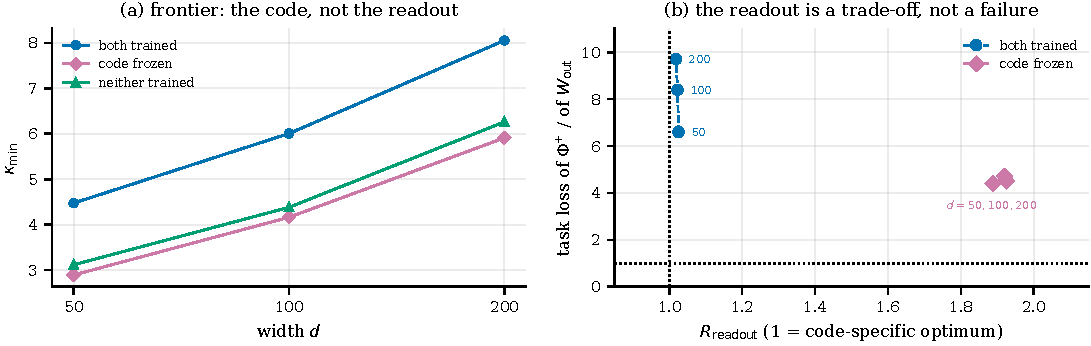
\includegraphics[width=\linewidth]{figures/fig6_frozen_encoder.pdf}
\caption{\textbf{Which half of the training does the work.} Medians over
\EeightSeeds{} models per arm and width. \textbf{(a)} The frontier tracks the code: training only the
readout leaves $\kappa_{\min}$ where an untrained code puts it --- below it, in fact --- while
training both lifts it at every width. \textbf{(b)} The same models placed by cross-talk against task
loss. The horizontal axis is $R_{\mathrm{readout}}$, so $1$ is the best readout \emph{of the code that
arm was given}; the vertical axis is how much lower the trained readout's own training loss is than
that optimum's. The frozen arm sits at nearly twice the cross-talk, which invites reading it as a
failed optimisation, but it beats the cross-talk optimum on the loss it trained under, so the
cross-talk is bought rather than lost. Its three widths coincide: neither coordinate moves as the
problem grows. The jointly trained arm is better on both axes at once and pulls further ahead with
width, so co-adaptation does not trade the two objectives against each other --- it aligns them.}
\label{fig:e8}
\end{figure}

The readout column is the surprise, and it is stable across width. The frozen arm trained
$W_{\mathrm{out}}$ for the full budget and ended at
$R_{\mathrm{readout}}=\EeightFrozenHundredRreadout{}$ at $d=100$ and
\EeightFrozenTwoHundredRreadout{} at $d=200$ --- nearly twice the cross-talk of the best readout
\emph{of the code it was given} --- while the jointly trained arm reaches
\EeightTrainedHundredRreadout{} and \EeightTrainedTwoHundredRreadout{}.

It is tempting to read that as gradient descent failing at the conditional problem, and it is not.
The cross-talk optimum is attained by $\Phi^{+}$ for \emph{every} code, so a readout with
$R_{\mathrm{readout}}$ near $1$ always exists and its existence settles nothing; what matters is
whether the arm's own objective prefers its $W_{\mathrm{out}}$ to that optimum. It does, decisively.
Scored under the loss the arm trained on, in its own post-ReLU representation, on fresh draws from a
seed no training used (\texttt{scripts/frozen\_readout\_tradeoff.py}), the frozen
$W_{\mathrm{out}}$ beats $\Phi^{+}$ by a factor of \EeightFrozenHundredTaskGain{} at $d=100$ and
\EeightFrozenTwoHundredTaskGain{} at $d=200$, on \EeightFrozenTwoHundredTaskWins{} of
\EeightSeeds{} models at each width. The cross-talk it gives up is bought, not lost. As a check on
the scoring, the untrained arm --- whose readout \emph{is} $\Phi^{+}$ --- returns a ratio of
\EeightRandomTwoHundredTaskGain{}. Figure~\ref{fig:e8}(b) places both arms in the two coordinates at
once, which is the only view in which the trade-off is visible as a trade-off.

So the two objectives genuinely pull apart on a fixed random code, and the contrast is about what
co-adaptation does to them rather than about optimisation difficulty: the jointly trained arm attains
$R_{\mathrm{readout}}=\EeightTrainedTwoHundredRreadout{}$ \emph{and} a task advantage of
\EeightTrainedTwoHundredTaskGain{} at $d=200$, so it does not trade one against the other at all,
while the frozen arm can only buy the second with the first. The joint arm's task advantage also
grows with width, \EeightTrainedFiftyTaskGain{} to \EeightTrainedHundredTaskGain{} to
\EeightTrainedTwoHundredTaskGain{}, where the frozen arm's is flat
(\EeightFrozenFiftyTaskGain{}, \EeightFrozenHundredTaskGain{},
\EeightFrozenTwoHundredTaskGain{}). Training the code appears to align the task objective with the
cross-talk objective; freezing it leaves them in conflict that no amount of readout training
resolves.

\paragraph{The frontier is now exact.} Earlier we reported $\kappa_{\min}$ over a subset of features
and called it an upper bound. Evaluating every feature of all 180 models shows the bound was tight:
the subset overestimated by \FullLfourTwoHundredSubsetOver{} on average at $d=200$ and never by more
than a tenth of a level. Its \emph{justification} is weaker than its accuracy, though. The subset was
chosen by Theorem~\ref{thm:arrow}, and that theorem is sufficient rather than necessary: on trained
codes it locates the true argmin in only \FullLfourTwoHundredArgminFound{} of 20 models at $d=200$,
where the true argmin sits at leverage rank \FullLfourTwoHundredArgminRankMed{} by median, outside
the window. On untrained codes it succeeds every time. Training pulls the lowest-leverage feature and
the worst-frontier feature apart, and the numbers above are the exact ones.

\paragraph{A fourth width, committed to in advance.} Before running it we extrapolated the frontier
from $d\in\{50,100,200\}$ and registered $\kappa_{\min}=\ScRegistered$ at $d=400$ in
\texttt{configs/e7\_stageC.json}. Then we ran the width --- \ScSeeds{} models per arm at $F=2d=800$,
same protocol --- and measured \ScMeasured{}, an error of \ScRegisteredErrorPct\% against the
registered value.

Two caveats on that number, both of which make it weaker than it first reads. The registered
extrapolation used the subset frontier, the only statistic available when it was written; refitting
on the exact frontier gives $\kappa_{\min}\propto d^{\ScFitExponent}$ and \ScPredicted{}, an error of
\ScPredErrorPct\%. We report the registered comparison as the primary one and the refit beside it,
because the refit was computed after seeing the measurement and is the more flattering of the two;
the three defensible pairings of predicted and measured all fall between $-2.2\%$ and $-2.6\%$, so
nothing here turns on the choice. And a prediction from three points fitting two parameters is a
weak instrument: it tests that the growth is regular, not that any particular law holds. We read the
result as a local rate rather than a law, because the exponent drifts downward across the four widths
and Section~\ref{sec:res-e6} explains why four points cannot separate the candidate shapes.

Two other things replicate at this width. The loss still decides the interface: $L^2$ reaches
$R_{\mathrm{geom}}=\ScLtwoRgeom$ with its frontier at \ScLtwoKappa, against $L^4$'s
\ScLfourRgeom{} and \ScLfourKappa{}, and the untrained code again sits near the floor at
\ScRandRgeom{} with a frontier of \ScRandKappa{}. And the matched decoder comparison continues in the
direction the smaller widths established, more sharply: at $d=400$ the network leads the affine probe
by \ScPrimDiff{} of a sparsity level ([\ScPrimCiLow, \ScPrimCiHigh]) in \ScPrimNetWins{} of
\ScSeeds{} models, where the three smaller widths gave a tie or a third of a level. Under the
conservative reading, in which the probe keeps the maximum over families evaluated on the test set,
the difference is \ScPrimTestMaxDiff{} --- so the ordering at this width does not depend on which of
the two defensible selection rules is used. Section~\ref{sec:probes} explains why this is a statement
about supervised fitting and not about what an affine readout can represent.

\paragraph{The margin over an untrained code is closing, and that is the finding of this width.}
Both frontiers grow with width, but not at the same rate: fitted over all four widths the trained
code gives $d^{\ScExpTrained}$ and the untrained one $d^{\ScExpRandom}$
(Fig.~\ref{fig:frontierscaling}a). The untrained exponent is the larger, so the advantage of training
is a decreasing function of width in both readings of ``advantage''. As a ratio it falls throughout
and faster each time: \MarginFiftyRatio, \MarginHundredRatio, \MarginTwoHundredRatio,
\MarginFourHundredRatio. In absolute sparsity levels --- the operationally meaningful unit, since the
frontier licenses supports up to $\lceil\kappa_{\min}\rceil-1$ --- it rises to a peak at $d=200$ and
then falls: \MarginFiftyGap, \MarginHundredGap, \MarginTwoHundredGap, \MarginFourHundredGap. The fall
is larger than the sampling noise: a two-sample bootstrap over models --- the arms are separately
trained, so the difference is between independent groups and not paired --- gives a drop of
\MarginDrop{} with
interval [\MarginDropCiLow, \MarginDropCiHigh], and the two widths' intervals do not overlap. Taken
at face value the two fitted laws meet near $d\approx\ScCrossing$.

We state this rather than the extrapolation. Four widths spanning a factor of eight cannot establish
where two rates cross, and $d\approx\ScCrossing$ is well outside the range measured. What the data
does support is narrower and still consequential: \emph{training buys frontier at every width we
measured, and the amount it buys stops growing by $d=400$.} A reader entitled to conclude that
gradient descent finds structurally better codes would want that margin to be at least stable in
width, and here it is not. Whether the trained code's deceleration reflects a real ceiling or the
fixed optimisation budget --- \EsevenSteps{} steps at every width, so the largest models get the
least optimisation per parameter --- this campaign cannot say, and it is the first thing a larger
budget should test.

\paragraph{And the shortcut has stopped being defensible.} The same width shows the subset
heuristic's justification collapsing, which is why every number in the two paragraphs above is the
exact minimum over all $F$ features. The mean overestimate grows \SubsetFiftyOver, \SubsetHundredOver,
\SubsetTwoHundredOver, \SubsetFourHundredOver; the median leverage rank of the true argmin grows
\SubsetFiftyRank, \SubsetHundredRank, \SubsetTwoHundredRank, \SubsetFourHundredRank; and at $d=400$
the subset locates the true argmin in \SubsetFourHundredFound{} of \ScSeeds{} trained models. The
error is still small in absolute terms, but it is one-sided and it is asymmetric between the arms:
untrained codes keep the true argmin at leverage rank 1, so their subset value \emph{is} exact, while
trained codes drift. A margin computed from subset values is therefore biased in favour of training
by an amount that grows with exactly the variable under study --- which is why we computed the exact
frontier for all four widths before making the claim above, and why we would not trust the shortcut
past $d=200$ in future work.

\begin{figure}[t]
\centering
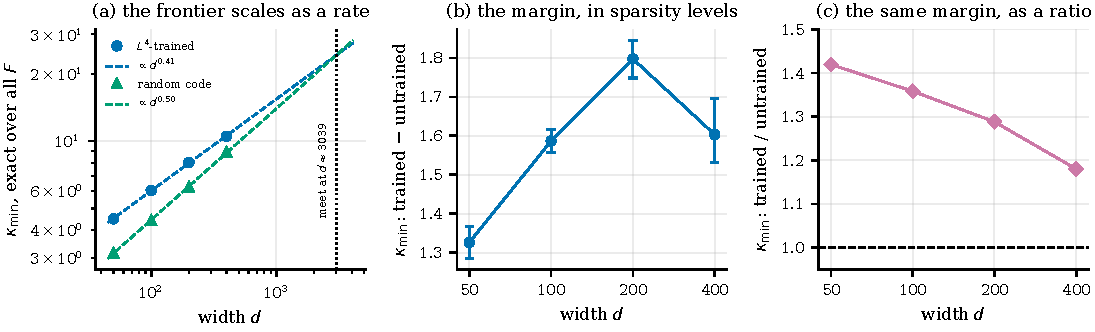
\includegraphics[width=\linewidth]{figures/fig7_frontier_scaling.pdf}
\caption{\textbf{The frontier's rate, and the margin it puts in question.} All values are the exact
$\kappa_{\min}$ over every one of the $F$ features, never the subset. \textbf{(a)} Both codes'
frontiers are close to straight on these axes over the four widths, and the untrained slope is the
steeper. The power-law fits meet near $d\approx\ScCrossing$, drawn to show what the two slopes imply
and not offered as a prediction: it lies far outside the measured range, and four points do not
identify the shape --- other forms fit as well and move the meeting point by a factor of two. The
robust statement is the ordering of the slopes, not where they cross. \textbf{(b)} The margin in sparsity
levels, with two-sample bootstrap intervals over models; it peaks at $d=200$ and the fall to $d=400$
exceeds the sampling noise. \textbf{(c)} The same margin as a ratio, which falls at every step. The
two panels are shown separately because they are the two honest readings of the same quantity and
they do not agree until $d=400$.}
\label{fig:frontierscaling}
\end{figure}

